\chapter{Aspect Théorique}

Dans la littérature, de nombreuses méthodes ont été utilisées pour déterminer le nombre de clusters optimaux. Parmi celles ci, nous pouvons citer:

\subsection*{La méthode de Milligan et Cooper (1985)}

La méthode de Milligan et Cooper (1985) consiste à maximisée suivant les valeurs de k l'indice suivant:
\[
CH(k)=\frac{B(k)/(k - 1)}{W(k)/(n - k)}
\]

Ou, où \(B(k)\) et \(W(k)\) sont respectivement la somme des carrés entre les groupes et la somme des carrés intra-groupes pour \(k\) groupes. Le nombre de clusters est donc donner par la valeur k qui maximise \(CH(k)\)

\subsection*{La méthode de  Krzanowski et Lai (1985)}

En se basant sur les travaux de Marriott (1971),Krzanowski et Lai (1985) proposent pour trouver le nombre de cluster optimal de maximiser la quantité \(KL(k)\) donnée par:

\[
KL(k)=\left|\frac{DIFF(k)}{DIFF(k + 1)}\right|
\]
Ou,
\[
DIFF(k)=(k - 1)^{2 / p}W_{k - 1}-k^{2 / p}W_{k}
\]

Le nombre de cluster est donc donné par la valeur de \(k\) qui maximise \(KL(k)\)

\subsection*{La méthode de Kaufman et Rousseeuw (1990)}

Kaufman et Rousseeuw (1990) proposent d'utiliser le coefficient de silhouette. Et de prendre la valeur de \(k\) qui maximise la moyenne des valeurs de \(s(i)\) pour l'ensemble des données . Pour une observation \(i\), \(s(i)\) est donné par:
\[
s(i)=\frac{b(i)-a(i)}{\max \{a(i), b(i)\}}
\]
Ou, \(a(i)\) la distance moyenne à d'autres points dans son groupe et \(b(i)\) la distance moyenne à tous les points du groupe le plus proche en dehors de son propre groupe

Il ressort donc que la plupart des méthodes présentes dans la littérature ne sont pas valables pour \(k=1\), autrement dit, elle ne permettent pas de dire s'il est possible ou non de faire un clustering. Robert Tibshirani et al.(2000) ont mis sur pied la méthode du Gap Statistique qui permet non seulement de déterminer le nombre de clusters optimale, mais aussi de tester s'il est nécessaire ou pas de créer des clusters.

\section{Gap Statistics}

Nos données ${x_{ij}}$ (où $i = 1, 2, ..., n$ et $j = 1, 2, ..., p$) sont constituées de $n$ observations indépendantes mesurées sur $p$ caractéristiques. Soit $d_{ii'}$ la distance entre les observations $i$ et $i'$. Le choix le plus courant pour $d_{ii'}$ est la distance euclidienne au carré :
$$
\sum_{j} (x_{ij} - x_{i'j})^{2}
$$
Supposons que nous avons regroupé les données en $k$ clusters $C_{1}, C_{2}, \ldots, C_{k}$, où $C_{r}$ représente les indices des observations dans le cluster $r$, et $n_{r} = \vert C_{r} \vert$.Soit
$$
D_{r}=\sum_{i, i' \in C_{r}} d_{i i'} \
$$ 
la somme des distances entre toutes les paires de points dans le cluster $r$, et définissons
$$
W_{k}=\sum_{r=1}^{k} \frac{1}{2 n_{r}} D_{r} \ (2)
$$
Tout d'abord, $D_{r} = \sum_{i, i' \in C_{r}} d_{ii'}$, qui représente la somme des distances entre toutes les paires de points dans le cluster $r$.
Ensuite, $W_{k} = \sum_{r = 1}^{k} \frac{1}{2n_{r}} D_{r}$, soit la somme, pour chaque cluster $r$ (avec $r$ variant de $1$ à $k$), du produit de $D_{r}$ par $\frac{1}{2n_{r}}$. Ici, $n_{r}$ est le nombre d'observations dans le cluster $r$ ($n_{r} = |C_{r}|$).
Lorsque la distance $d$ est la distance euclidienne au carré, $W_{k}$ représente la somme des carrés des distances intra-clusters autour des moyennes de chaque cluster, où le coefficient $2$ assure la cohérence de ce calcul. Dans cette notation, la taille de l’échantillon $n$ est omise. En général, plus la valeur de $W_{k}$ est petite, plus les points au sein des clusters sont rapprochés, ce qui indique potentiellement une meilleure qualité de clustering. Cette mesure est utilisée pour évaluer la qualité du clustering en fonction du nombre de clusters $k$ et joue un rôle important dans le calcul de la statistique de l’écart (Gap Statistic) dans les étapes ultérieures.

Prenons deux exemples simples. Considérons un cluster $r$, où $D_r$ représente la somme des distances entre toutes les paires de trois observations dans ce cluster. Supposons simplement que la distance entre chaque paire de points est la même, afin de simplifier la compréhension. Étant donné que chaque distance entre deux points est comptée deux fois (par exemple, la distance entre le point $i$ et le point $i'$, ainsi que celle entre $i'$ et $i$), cela équivaut à deux fois la somme des longueurs des arêtes.
\begin{figure}[H]
    \centering
    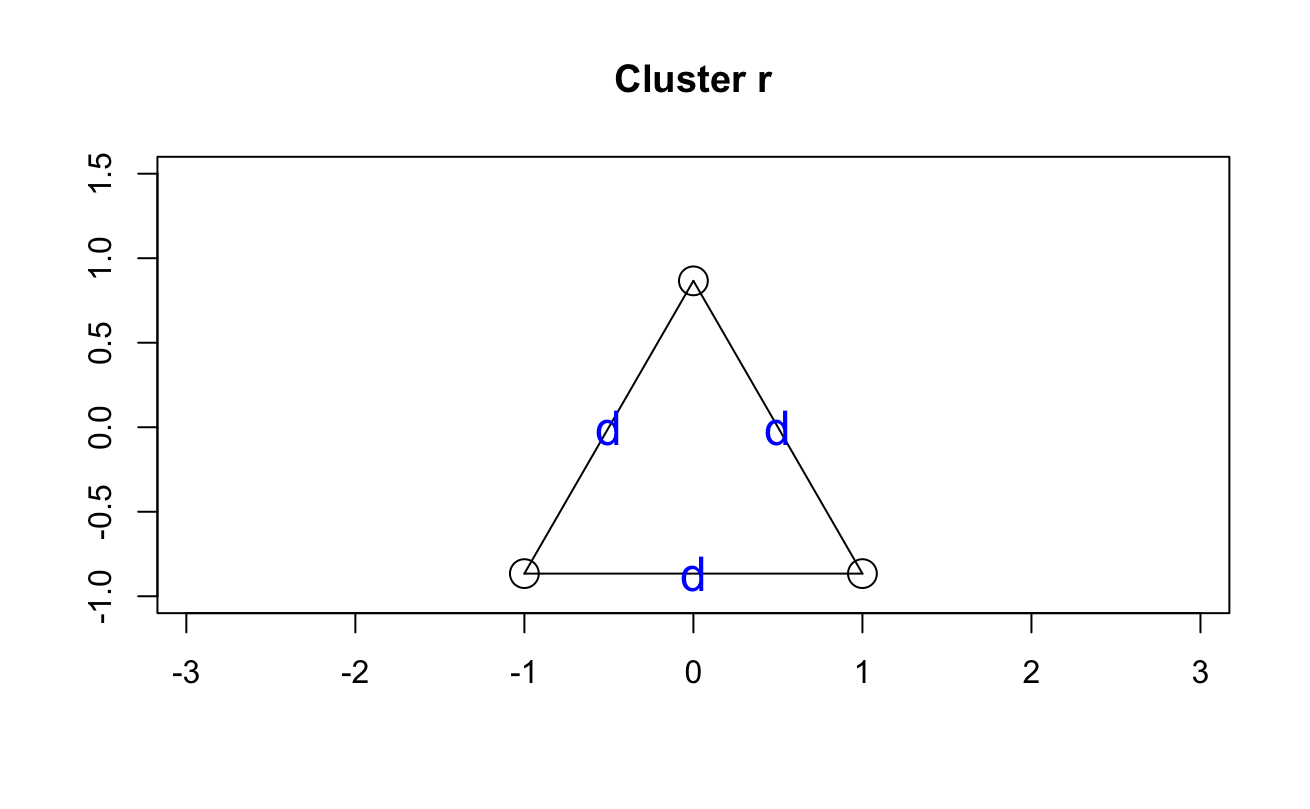
\includegraphics[width=1\linewidth]{images/cluster r.png}
    \caption{Exemple K = 1}
    \label{fig:enter-label}
\end{figure}

$$
D_r = D \times 2 \times 3
$$

Prenons un autre exemple pour $W_k$ où $k = 3$.
\begin{figure}[H]
    \centering
    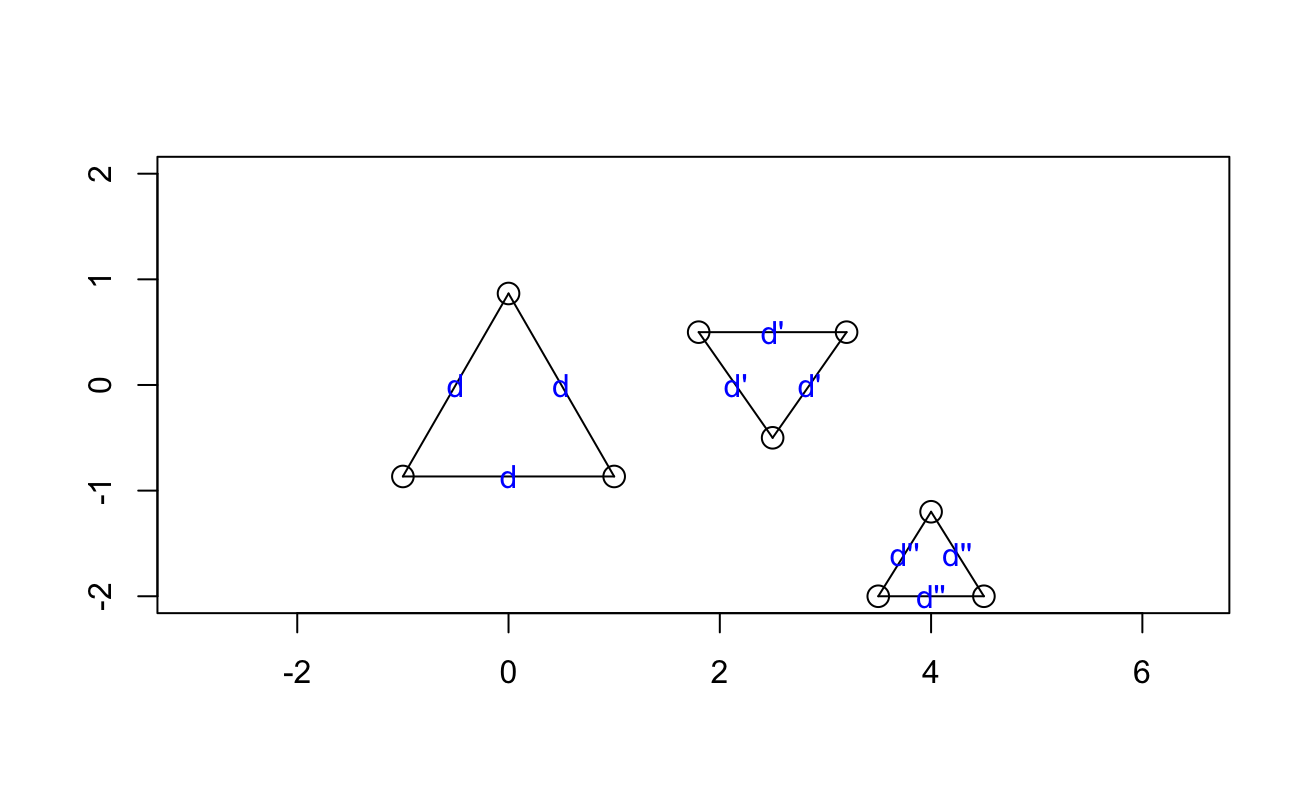
\includegraphics[width=0.9\linewidth]{images/3triangles.png}
    \caption{Exemple K = 3}
    \label{fig:enter-label}
\end{figure}
$$
W_k = \sum_{r=1}^{k = 3} \frac{D_r}{2 n_r} =\frac{ d \times 2 \times 3 + d' \times 2 \times 3 + d'' \times 2 \times 3}{2\times3}
$$

\begin{figure}[H]
    \centering
    % 左侧图片
    \begin{subfigure}[b]{0.45\linewidth}
        \centering
        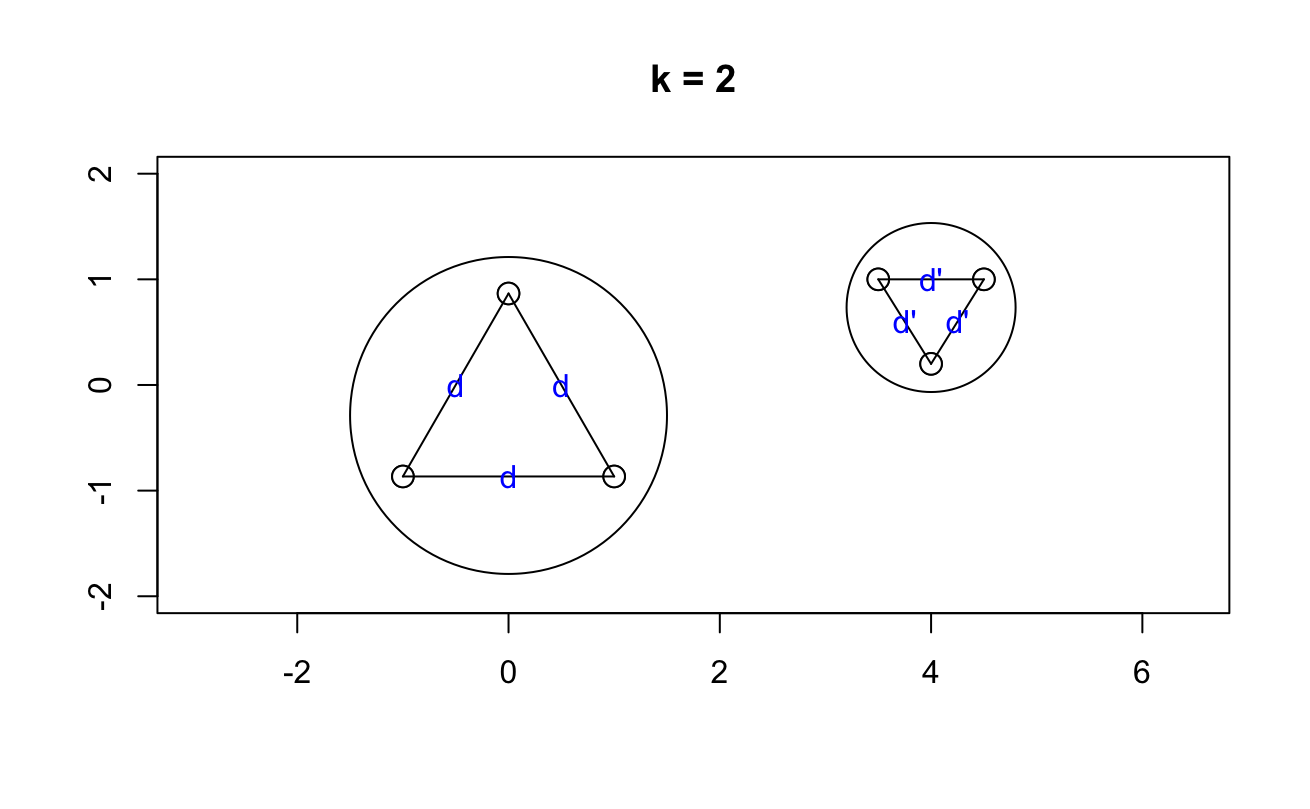
\includegraphics[width=\linewidth]{images/2k.png}
        \caption{K = 2}
        \label{fig:2k}
    \end{subfigure}
    \hspace{0.05\linewidth} % 两张图片之间的间隔
    % 右侧图片
    \begin{subfigure}[b]{0.45\linewidth}
        \centering
        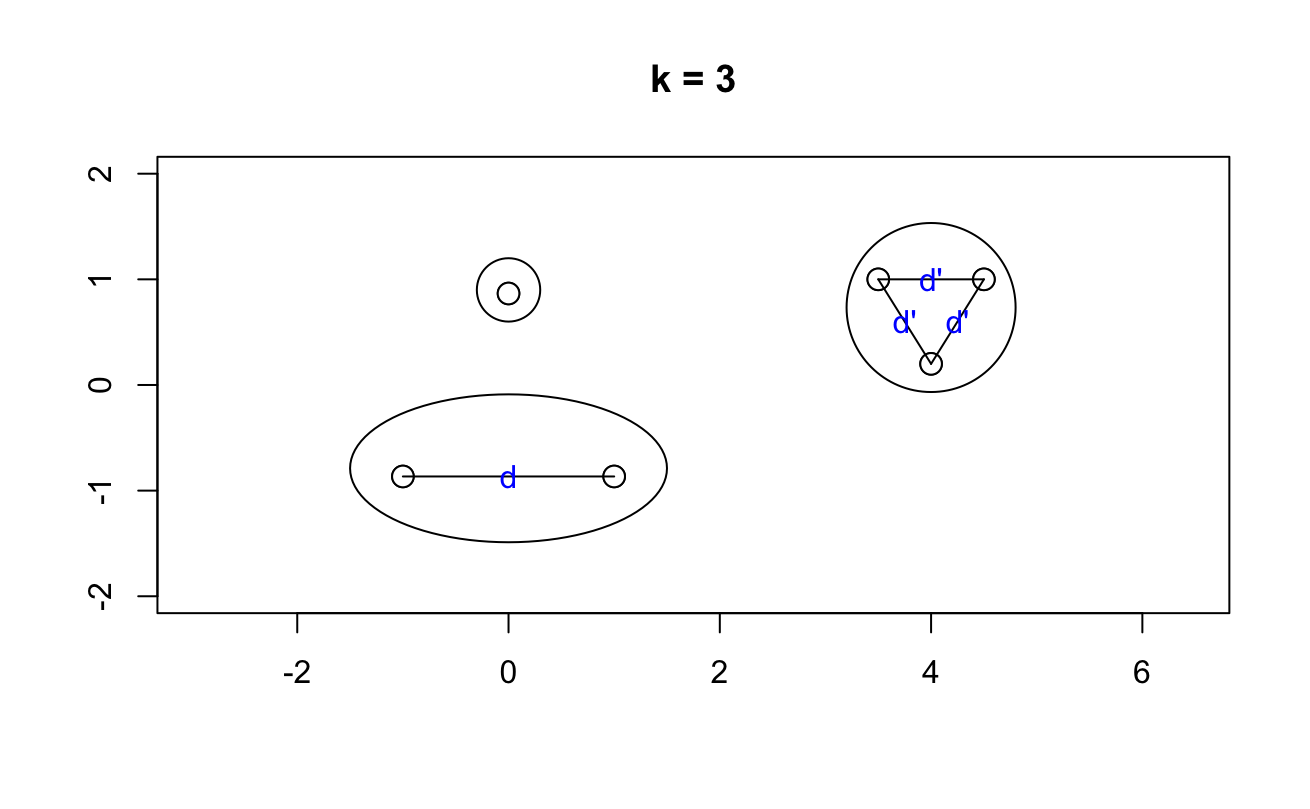
\includegraphics[width=\linewidth]{images/3k.png}
        \caption{K = 3}
        \label{fig:3k}
    \end{subfigure}
    
    \caption{}
    \label{fig:side-by-side}
\end{figure}

Dans cet exemple simple, si le nombre de clusters dépasse 2 à 3, alors la distance moyenne $W_k$ reste inchangée.
$$
\begin{aligned}
W_2 &= \sum_{r=1}^{2} \frac{D_r}{2 n_r} =\frac{ d \times 2 \times 3 + d' \times 2 \times 3}{2\times3} = d+d'\\
 W_3 &=\sum_{r=1}^{3} \frac{D_r}{2 n_r} =0+ \frac{d \times 2 \times 2}{2 \times 2 }+\frac{d' \times 2 \times 3 }{2 \times 3 } = d+d'
\end{aligned}
\Longrightarrow W_2 = W_3
$$

En comparant le graphique de $\log (W_{k})$ avec la valeur attendue des données sous une distribution de référence appropriée pour l'hypothèse nulle, on peut ainsi le standardiser.Ensuite, notre estimation du nombre optimal de clusters est la valeur de $k$ pour laquelle la diminution de $\log (W_{k})$ par rapport à cette courbe de référence est la plus importante.

Par conséquent, nous définissons , pour chaque $k \in \mathbb{N_*}$:

$$
Gap_{n}(k) = E_{n}^{*}\left\{\log \left(W_{k}\right)\right\}-\log \left(W_{k}\right) \ (3) 
$$


\begin{figure}[H]
    \centering
    % 第一排图片
    \begin{subfigure}[b]{0.45\linewidth} % 左侧子图
        \centering
        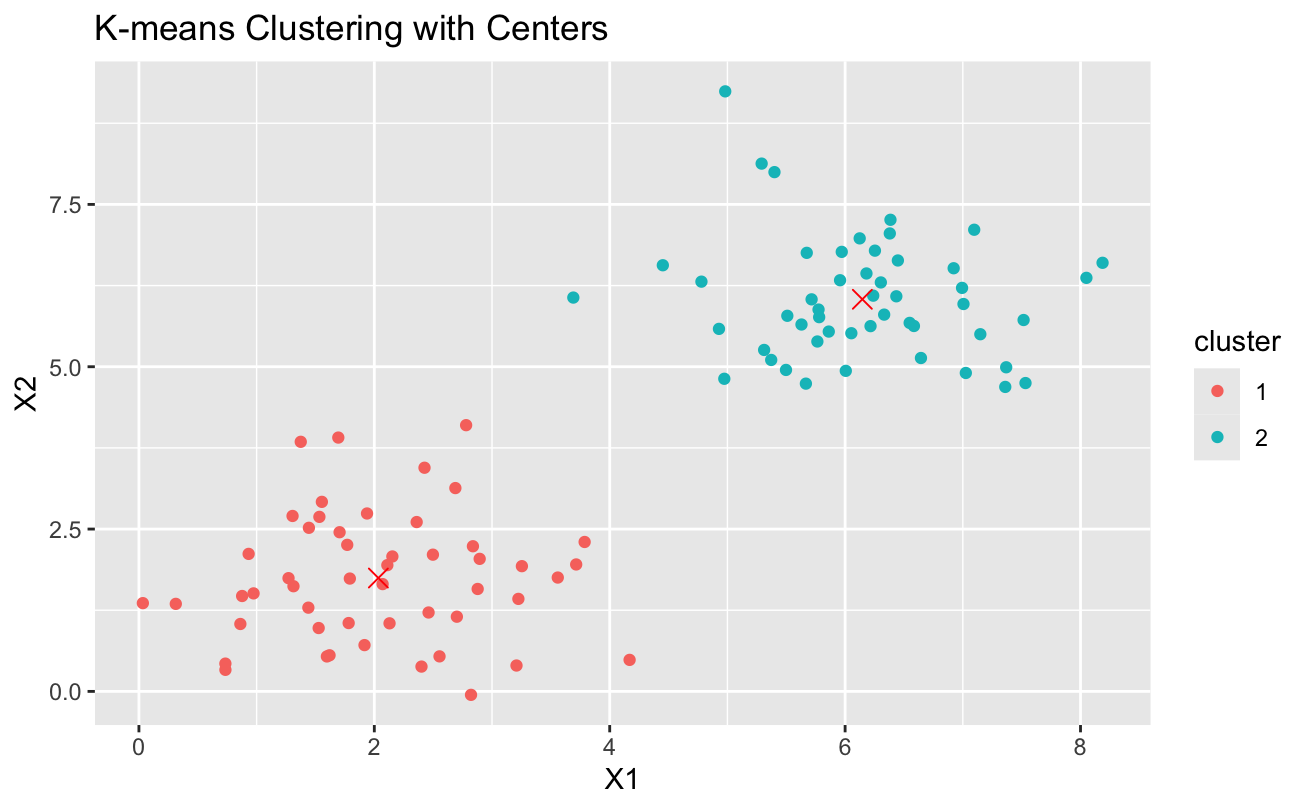
\includegraphics[width=\linewidth]{images/A.png}
        \caption{Nuage}
        \label{fig:image-A}
    \end{subfigure}
    \hspace{0.05\linewidth} % 两个子图之间的间隔
    \begin{subfigure}[b]{0.45\linewidth} % 右侧子图
        \centering
        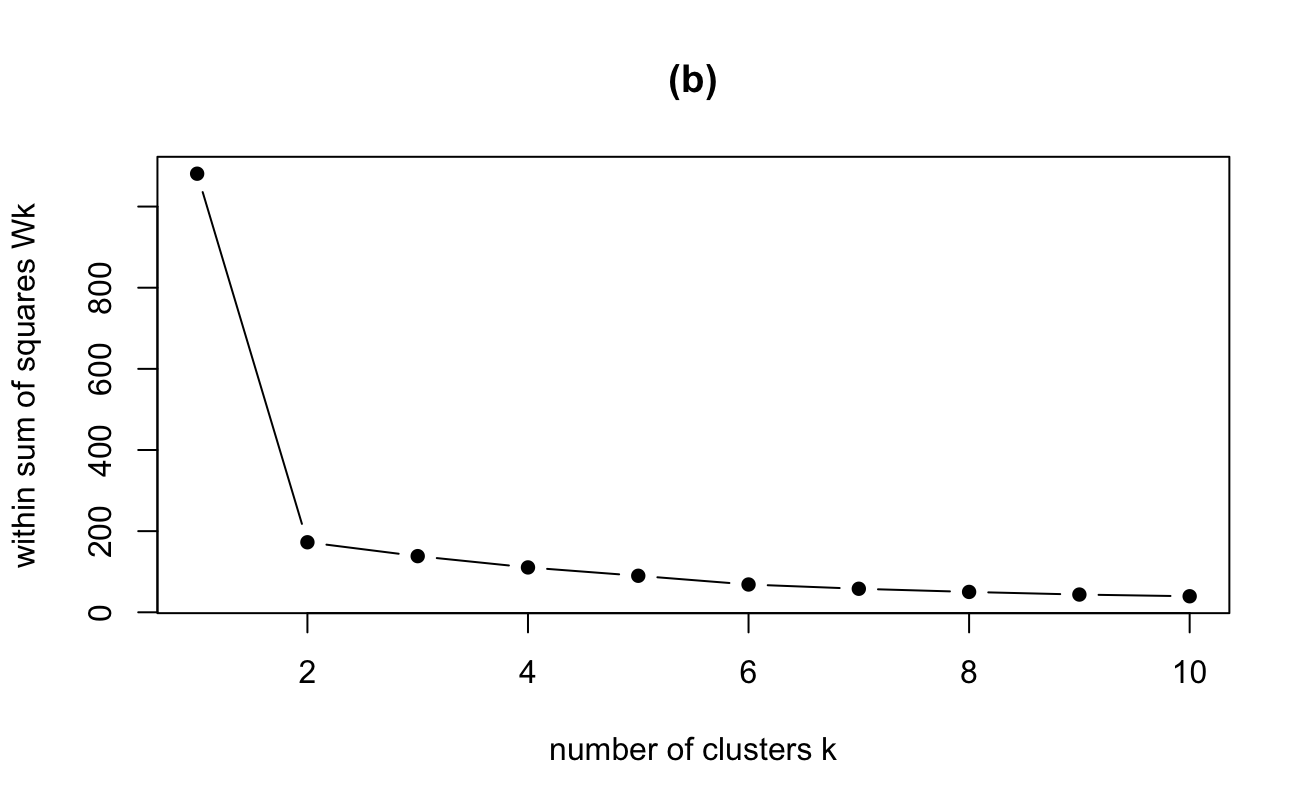
\includegraphics[width=\linewidth]{images/B.png}
        \caption{$W_k$}
        \label{fig:image-B}
    \end{subfigure}
    
    % 第二排图片
    \vspace{0.5cm} % 第一排和第二排之间的间隔
    \begin{subfigure}[b]{0.45\linewidth} % 左侧子图
        \centering
        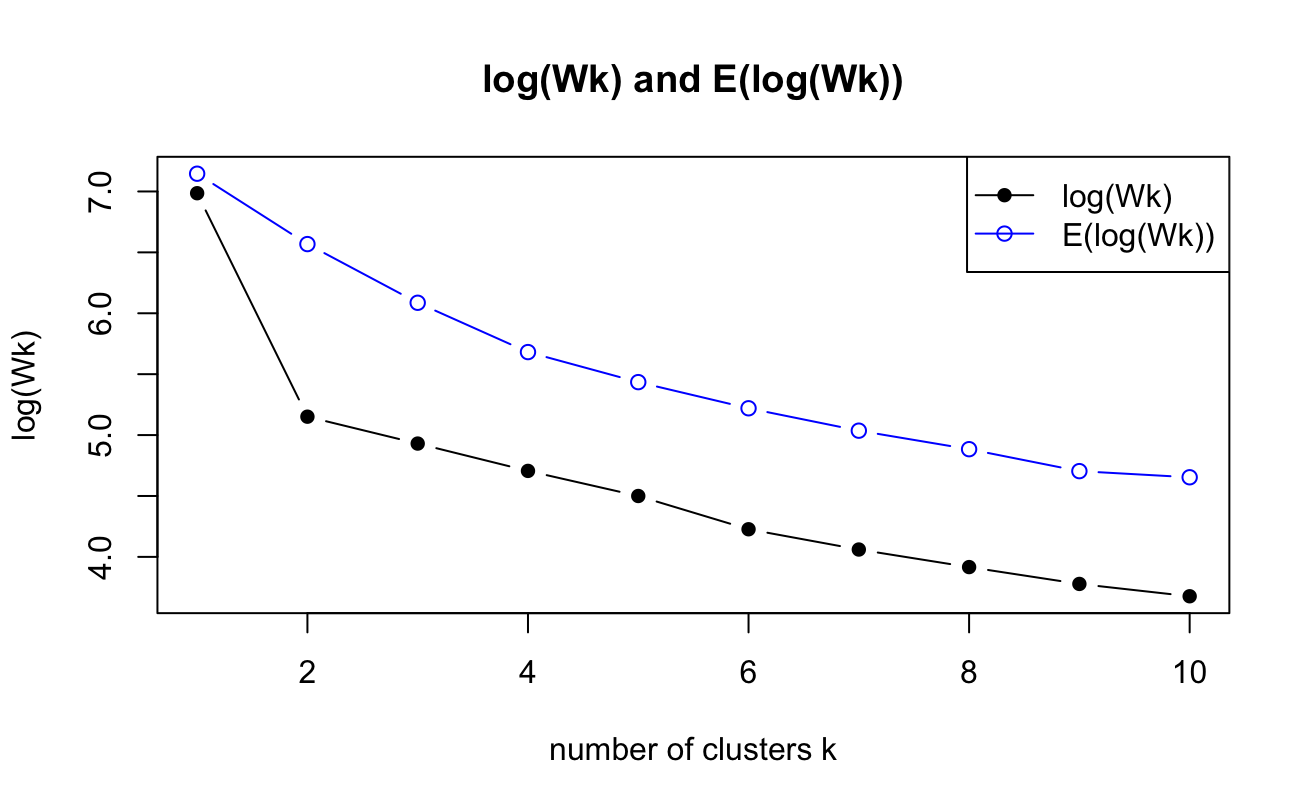
\includegraphics[width=\linewidth]{images/C.png}
        \caption{Espérence et logarithme}
        \label{fig:image-C}
    \end{subfigure}
    \hspace{0.05\linewidth} % 两个子图之间的间隔
    \begin{subfigure}[b]{0.45\linewidth} % 右侧子图
        \centering
        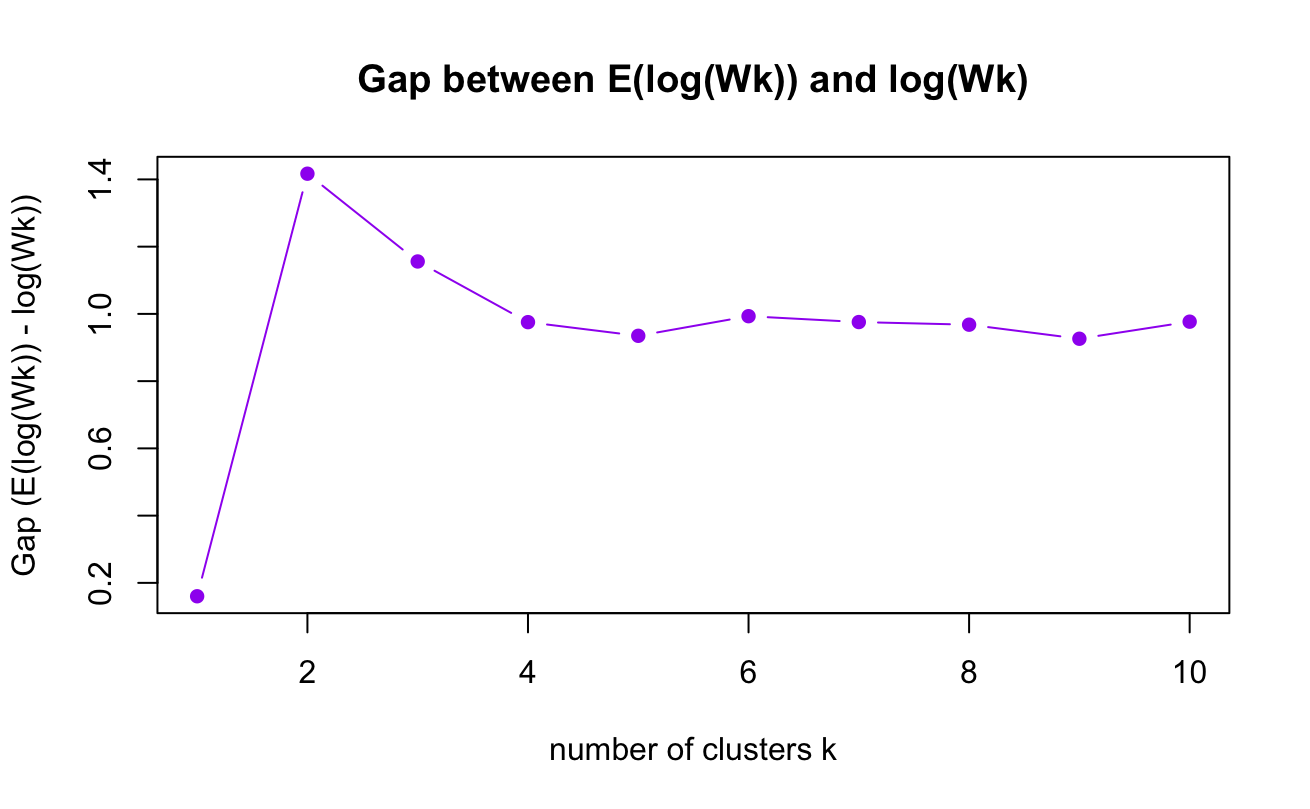
\includegraphics[width=\linewidth]{images/D.png}
        \caption{Le Gap}
        \label{fig:image-D}
    \end{subfigure}
    
    \caption{}
    \label{fig:four-images}
\end{figure}

\section{Reference distribution}

Pour transformer le Gap Statistic en procédure opérationnelle, nous devons trouver une distribution de référence appropriée et évaluer la distribution d'échantillonnage du Gap Statistic.

\subsection{Principe de génération}

Nous supposons que le dataset d'échantillons est $X$, avec $n$ samples, $p$ features.

$$
\text{X} = 
\begin{bmatrix}
  & x_{1,1} & \cdots & \cdots & x_{1,p} \\
  & \vdots & \ddots &  \ddots &\vdots \\
  & x_{i,1} & \cdots  & \cdots & x_{i,p} \\
  & \vdots & \ddots  & \ddots & \vdots \\
  & x_{n,1} & \ddots & \cdots & x_{n,p} \\
\end{bmatrix}
\text{n samples, p features}
$$

Pour chaque feature, il doit y avoir une valeur minimale et une valeur maximale. Par exemple, la première feature : $X_1 \in [x_{1,min},x_{1,max}]$.

Générons de manière aléatoire d'une distribution de référence par une distribution continue uniforme, nous obtenons :

$$
\text{$X'_1$} = 
\begin{bmatrix}
  & x'_{1,1} \\
  & \vdots  \\
  & \vdots \\
  & x'_{n,1} \\
\end{bmatrix}
\text{n samples}
$$ 

où $x'_{i,1} \in [x_{1,min},x_{1,max}]$.

Pour les autres features, nous les générons de la même manière, alors nous obtenons la distribution de référence $X'$ :

$$
\text{X'} = 
\begin{bmatrix}
  & x'_{1,1} & \cdots & \cdots & x'_{1,p} \\
  & \vdots & \ddots &  \ddots &\vdots \\
  & x'_{i,1} & \cdots  & \cdots & x'_{i,p} \\
  & \vdots & \ddots  & \ddots & \vdots \\
  & x'_{n,1} & \ddots & \cdots & x'_{n,p} \\
\end{bmatrix}
\text{n samples, p features}
$$

Nous désignons par $S^{p}$ l'ensemble de ces distributions à composante unique (ou variables aléatoires) sur $R^{p}$.

Pour voir comment trouver une distribution de référence appropriée, considérons un instant la version de la population correspondant au Gap Statistic dans le cas du regroupement par K-means :
$$
g(k)=\log\left\{\frac{MSE_{X^{*}}(k)}{MSE_{X^{*}}(1)}\right\}-\log\left\{\frac{MSE_{X}(k)}{MSE_{X}(1)}\right\}
$$ où $MSE_{X}(k)=E(\min_{\mu\in A_{k}}\|X - \mu\|^{2})$.

Le gap statistic compare les performances du modèle null (un cluster) à celles des modèles alternatifs ($k > 1$) en mesurant la réduction de la variance intra-cluster. $A_{k}\subset R^{p}$ est un ensemble de $k$-points minimisant cette variance. La statistique est normalisée pour que $g(1)=0$, facilitant la comparaison entre le modèle nul et les modèles avec plusieurs clusters.

Selon l'article, nous introduisons maintenant deux théorèmes sur la distribution de référence.

Pour des lois univarié, la distribution de référence est donnée par le théorème suivant:

\textbf{Théorème 1}. Soit \(p = 1\). Alors, pour tous \(k \geq 1\).

\begin{equation}
\inf_{X \in S^p} \left\{ \frac{MSE_{X}(k)}{MSE_{X}(1)} \right\} = \frac{MSE_{U}(k)}{MSE_{U}(1)}
\end{equation}

Ou , \(S^{p}\) représente l'ensemble des distributions (ou variables aléatoires) à une seule composante dans \(R^{p}\).

Ce théorème montre que, dans le cas univarié, la distribution de référence est donnée par la loi uniforme \(U = U[0,1]\). 

Dans le cas multidimensionnel, déterminer la loi de référence n'est plus aussi simple comme le montre le résultat suivant:

\textbf{Théorème 2}. Si \(p > 1\), alors,aucune distribution \(U \in S^{p}\) dont le  support est différent d'une droite, ne peut satisfaire l'équation (1).
Pour $p>1$, il n'existe aucune distribution de référence $U \in S^{p}$, sauf si son support est réduit à un sous-ensemble dégénéré (ex. une ligne droite).

Donc, en dimensions élevées, on ne peut pas utiliser une méthode générique pour comparer les modèles. Cela limite l'applicabilité directe du Gap Statistic telle qu'elle est définie pour les cas univariés.

Une solution consiste à générer des données de référence à partir de l'estimateur du maximum de vraisemblance (MLE) sous contrainte de log-concavité.

En dimension 1, cette estimation peut être réalisée à l'aide d'algorithmes d'approximation convexes.

On constate alors que dans le cas multidimensionnelle, on est pas capable de trouver directement la distribution de référence. Robert \textit{Tibshirani et al.(2000)} en se basant sur le théorème 1 proposent donc d'utiliser une méthode numérique basée sur la \textit{simulation de Monté Carlo}.


\subsection{Méthode Numérique pour l'estimation de de la distribution de référence}

\begin{enumerate}[label=(\alph*)] % Définit le style de numérotation
	\item Pour chaque caractéristique de référence, générer des valeurs pour cette caractéristique de manière uniforme dans la plage des valeurs observées pour cette caractéristique.
	
	\item Générer les caractéristiques de référence à partir d'une distribution uniforme dans un rectangle aligné avec les composantes principales des données. Plus précisément, si \(X\) est notre matrice de données de dimension \(n \times p\), supposons que les moyennes des colonnes sont égales à \(0\) et calculons la décomposition en valeurs singulières : 
	\[
	X = UDV^{T}.
	\]
	Nous effectuons une transformation : 
	\[
	X' = XV,
	\]
	puis, comme dans la méthode (a), nous tirons des caractéristiques uniformes \(Z'\) dans la plage des valeurs des colonnes de \(X'\). Enfin, nous effectuons une transformation inverse : 
	\[
	Z = Z'V^{T},
	\]
	pour obtenir les données de référence \(Z\)
\end{enumerate}

La méthode (a) a l'avantage de la simplicité. La méthode (b) prend en compte la forme de la distribution des données et, tant que la méthode d'agrégation elle-même est invariante, peut rendre l'ensemble du processus invariant par rotation.

Dans chaque cas, nous estimons \(E_{n}^{*}\{\log (W_{k})\}\) en prenant la moyenne de \(B\) copies de \(\log (W_{k}^{*})\), où chaque \(\log (W_{k}^{*})\) est calculé à partir d'un échantillon de Monte Carlo $X_{1}^{*}, \ldots, X_{n}^{*}$ tiré de notre distribution de référence. Enfin, nous devons évaluer la distribution d'échantillonnage de la statistique d'écart. Soit \(sd(k)\) l'écart type de \(B\) répétitions de Monte Carlo des \(\log (W_{k}^{*})\). En outre, compte tenu de l'erreur de simulation dans \(E_{n}^{*}\{\log (W_{k})\}\), nous obtenons la quantité
\[
s_{k}=\sqrt{(1 + 1 / B)} sd(k)
\]

\subsection{Algorithme pour le choix du nombre de cluster}
La procédure est la suivante:

\textbf{Étape 1} : Effectuer une agrégation des données d'observation en faisant varier le nombre total de groupes de \(k = 1\), \(2\), \(\ldots\), \(K\), afin d'obtenir les valeurs de la mesure de dispersion intra-groupe \(W_{k}\) (où \(k = 1\), \(2\), \(\ldots\), \(K\)).

\textbf{Étape 2} : Utiliser l'un des deux choix de distribution uniforme mentionnés ci-dessuspour générer \(B\) ensembles de données de référence et effectuer une agrégation pour chacun de ces ensembles de données de référence, afin d'obtenir les valeurs de la mesure de dispersion intra-groupe \(W_{k b}^{*}\) (où \(b = 1\), \(2\), \(\ldots\), \(B\), \(k = 1\), \(2\), \(\ldots\), \(K\)). Calculer la statistique d'écart (estimée)
\[
Gap(k)=\frac{1}{B}\sum_{b}\log\left(W_{k b}^{*}\right)-\log\left(W_{k}\right)
\]

\textbf{Étape 3} : Soit \(\tilde{I}=\frac{1}{B}\sum_{b}\log (W_{k b}^{*})\), calculer l'écart type
\[
sd_{k}=\left[\frac{1}{B}\sum_{b}\left\{\log (W_{k b}^{*}) - \overline{I}\right\}^{2}\right]^{\frac{1}{2}}
\]

En utilisant cette condition, nous choisissons la taille du groupe \(k\) comme étant la plus petite valeur de \(k\) qui satisfait \(Gap(k) \geq Gap(k + 1) - s_{k + 1}\)
% Ajoutez d'autres sections ici si nécessaire



